\section{Aufbau}
\label{sec:Aufbau}
\begin{wrapfigure}[14]{r}{5cm}
\centering
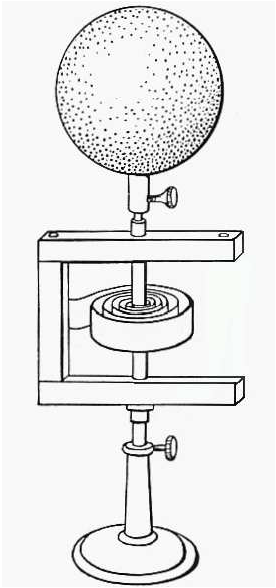
\includegraphics[width=3cm]{content/images/Drillachse.png} 
\caption{Drillachse\cite{V101}}
\label{fig:Drillachse}
\end{wrapfigure}
Als schwingendes System wird eine Drillachse (Abbildung \ref{fig:Drillachse}) verwendet. Sie besitzt ein Eigenträgheitsmoment $I_.D$ und eine Winkelrichtgröße $D$.
Der zu untersuchende Körper wird auf die Drillachse gespannt und schwingt aufgrund der Spiralfeder, welche eine rückwirkende Kraft ausübt, mit der Periodendauer $T$.